\section{Method}
\label{sec:method}

We consider a frozen autoregressive Transformer with $L$ layers and $H$ KV heads. Prefilling a context of $T$ tokens, $c=(c_1,\ldots,c_T)$, produces a cache $\mathcal{C}(c)$ and hidden representations $X^{\ell}\in\mathbb{R}^{T\times d}$. Compression is applied after this prefill, producing a cache for subsequent questions. A selector with parameters $\theta$ assigns a score $s_{\ell h i}$ to each context entry. Compression retains a subset of the original KV pairs according to these scores and a retention budget $\rho$. The selector observes the context before the downstream question is supplied. System-prefix entries and subsequently appended question and answer tokens lie outside the context budget.

\subsection{Fast KVzip Gating Mechanism}
\label{sec:gate}

Fast KVzip predicts KV importance from token representations using a low-dimensional sink-attention gate~\citep{kim2026fastkvzip}. Fix a layer $\ell$ and KV head $h$, and write $x=x_i^{\ell}$. Suppressing these indices on the projection parameters, the gate forms a key and $G$ queries, where $G$ is the number of query heads sharing the KV head:
\begin{equation}
    \widehat{\mathbf q}_j=\operatorname{RMSNorm}_{\ell}^{q}\!\left(xW_j^q+\mathbf b_j^q\right),\qquad
    \widehat{\mathbf k}=\operatorname{RMSNorm}_{\ell}^{k}\!\left(xW^k\right),
    \label{eq:gate-features}
\end{equation}
with $W_j^q,W^k\in\mathbb{R}^{d\times d_g}$ and gate width $d_g$. RMSNorm rescales each projected vector by its root-mean-square magnitude and applies learned featurewise scales. These are auxiliary gate features.

Let $\boldsymbol\kappa_1,\ldots,\boldsymbol\kappa_S\in\mathbb{R}^{d_g}$ be learned reference keys, shared across token positions. With the token-key logit $a_j=\langle\widehat{\mathbf q}_j,\widehat{\mathbf k}\rangle/\sqrt{d_g}+b_j$ and learned scalar bias $b_j$, the gate used here is
\begin{equation}
    s_{\ell h i}=g_{\ell h}(x_i^{\ell})=
    \frac{1}{G}\sum_{j=1}^{G}
    \frac{\exp(a_j)}{\exp(a_j)+\sum_{m=1}^{S}
    \exp\!\left(\langle\widehat{\mathbf q}_j,\boldsymbol\kappa_m\rangle/\sqrt{d_g}\right)}.
    \label{eq:fastkvzip-gate}
\end{equation}
Each fraction measures the attention mass assigned to the token's key in competition with the reference keys; averaging yields one importance score per KV head. The frozen Transformer supplies contextual representations, which this gate scores separately at each position. Our graph module enriches these representations through message passing before applying the same mapping $g_{\ell h}$.

\subsection{Graph-Based Token Mixing}
\label{sec:mixing}

\subsubsection{Graph Construction}

We partition the context into contiguous blocks $\mathcal{B}$ and apply the same selector parameters to each block. A single block can also cover the entire context. For one block $b\in\mathcal{B}$ of $T_b=|b|$ tokens, suppress the layer and head indices and write its representations as $X\in\mathbb{R}^{T_b\times d}$. Learned projections $W_a,W_v\in\mathbb{R}^{d\times r}$ produce relation features $U$ and message features $R$:
\begin{equation}
    U=XW_a,\qquad R=XW_v,\qquad A=\frac{1}{T_b}UU^{\top}.
    \label{eq:graph}
\end{equation}
Here $A_{ij}$ is the weight of the connection between tokens $i$ and $j$. The relation projection is learned across contexts, while the graph is recomputed from the representations of each input. Every layer--KV-head pair has its own projections. The adjacency is symmetric, can contain signed weights, and includes self-connections. These weights define learned feature interactions rather than probabilities or prescribed semantic relations.

\subsubsection{Message Passing and Retention Scores}

With $W_o\in\mathbb{R}^{r\times d}$, we aggregate messages and form a residual update:
\begin{equation}
    P=ARW_o,\qquad
    X'=X+\alpha\,\operatorname{LeakyReLU}\!\left(\operatorname{BatchNorm}(P)\right),\qquad
    s_{\ell h i}=g_{\ell h}(x'_i).
    \label{eq:mixer}
\end{equation}
BatchNorm~\citep{ioffe2015batchnorm} uses the current block's token statistics during both training and inference. The scalar $\alpha$, normalization parameters, and message projections are specific to each layer--KV-head pair. This update follows the aggregation-and-update structure of message-passing networks \citep{gilmer2017mpnn,xu2019gin}; the learned weighted graph specifies which token features contribute to each message. We evaluate message passing in factorized form without constructing the adjacency matrix, giving a cost linear in block length for fixed feature dimensions (Appendix~\ref{app:factorized}).

The residual changes only the auxiliary representations used for scoring. The language model's hidden states and retained KV vectors are not replaced by mixed features. Scores from all blocks are concatenated before eviction, so graph blocks do not impose separate retention quotas. Given a retention ratio $\rho$, a uniform per-head budget retains the $k=\max(1,\lfloor\rho T\rfloor)$ highest-scoring context entries in each layer and KV head. The scores also support a shared budget across layers and heads, allowing nonuniform retention. Selected entries keep their original order and positional information. Block boundaries restrict the selector's message passing, while its input representations retain the contextual information supplied by the frozen Transformer.

\begin{figure}[t]
    \centering
    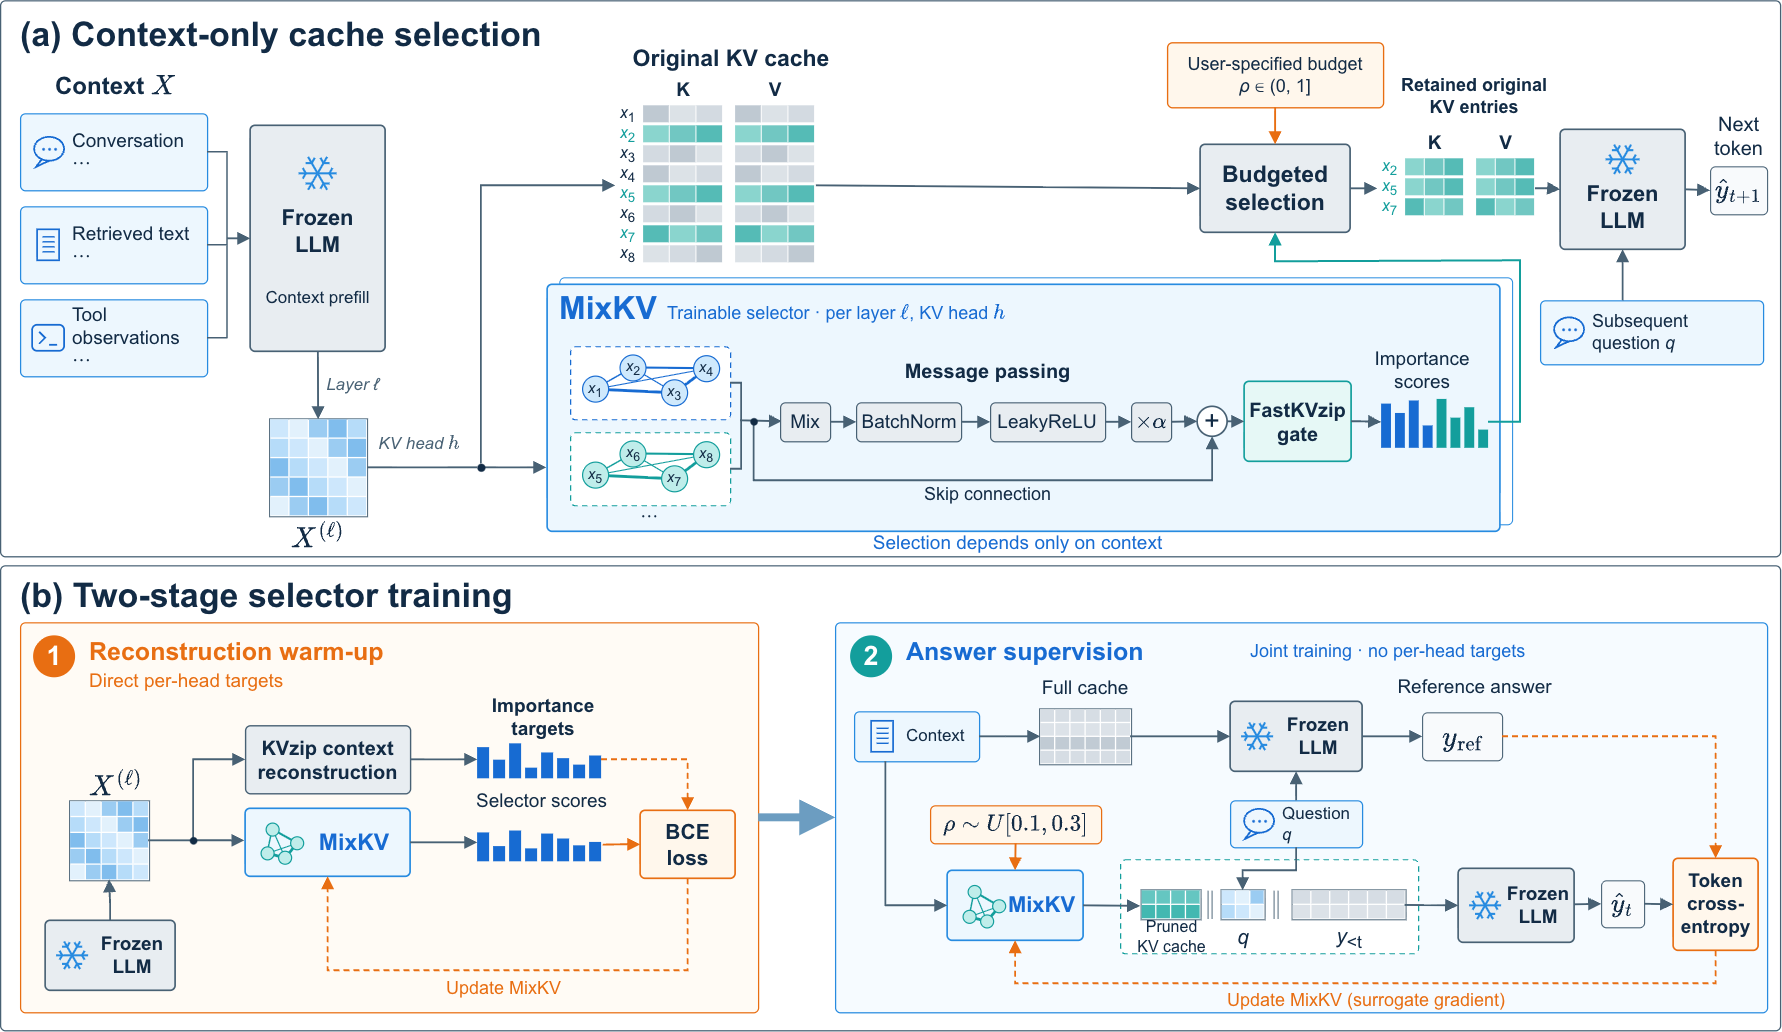
\includegraphics[width=\linewidth]{figures/mixkv-overview.png}
    \caption{\textbf{MixKV architecture and training.}
    (a) A trainable selector mixes context-token representations through message passing and scores them with a Fast KVzip gate. Budgeted selection retains original KV entries before a subsequent question is supplied.
    (b) Reconstruction-score supervision warms up the selector, followed by answer supervision from the frozen full-cache model using a straight-through surrogate. The language model remains frozen in both stages.}
    \label{fig:overview}
\end{figure}

\subsection{Two-Stage Training}
\label{sec:training}

\subsubsection{Stage 1: Reconstruction-Supervised Warm-Up}

KVzip computes an importance target $t_{\ell h i}\in[0,1]$ from the maximum attention received by a cached entry during context reconstruction, aggregating over reconstruction positions and the query heads that share that KV head \citep{kim2025kvzip}. Following Fast KVzip, we use these scores as continuous targets for binary cross-entropy. For a collection of training blocks, the objective is
\begin{equation}
    \mathcal{L}_{\mathrm{warm}}=
    -\frac{1}{|\mathcal{B}|LH}\sum_{b\in\mathcal{B}}\sum_{\ell,h}
    \frac{1}{T_b}\sum_{i\in b}
    \left[t_{\ell h i}\log s_{\ell h i}+(1-t_{\ell h i})\log(1-s_{\ell h i})\right].
    \label{eq:warmup}
\end{equation}
Both the graph mixer and gate are trained, with the gate optionally initialized from Fast KVzip. Reconstruction supervision supplies a direct target for each cache entry and gives the selector an informed starting point. These targets express the reconstruction procedure's assessment of importance; reproducing them alone does not directly optimize answers generated from a compressed cache.

\subsubsection{Stage 2: Answer Supervision}

For a context--question pair $(c,q)$, the frozen language model with its full cache generates a reference answer $y^*$. We then compress the context cache using the selector and train on the reference answer under teacher forcing:
\begin{equation}
    \mathcal{L}_{\mathrm{ans}}(\theta)=
    -\frac{1}{|y^*|}\sum_{t=1}^{|y^*|}
    \log p_{\phi}\!\left(y_t^*\mid q,y_{<t}^*,\mathcal{C}_{\theta}(c;\rho)\right),
    \label{eq:answerloss}
\end{equation}
where $\phi$ denotes the frozen language-model parameters. Only answer tokens contribute prediction loss. The question and reference prefix condition the prediction, and gradients update the mixer and gate. We vary $\rho$ across training examples, either by sampling a retention interval or by following a decreasing schedule. This stage aligns cache selection with the model's ability to predict its full-cache answers, rather than requiring continued agreement with reconstruction scores. It uses reference sequences, not a loss matching the teacher's complete output distribution. Answer supervision is query-dependent during training, but the learned selector remains a function of the context alone.

To train through hard top-$k$ selection, we use a straight-through surrogate that preserves the retained KV entries in the forward pass while supplying score gradients during backpropagation (Appendix~\ref{app:surrogate}). We then recompute the selector one graph block at a time and replay these score gradients, limiting live selector activations to one block (Appendix~\ref{app:replay}).
